\documentclass{beamer}
\usetheme{Goettingen}

\usepackage{hyperref}
\usepackage{fancybox}


\title[Bash]{Introduction to Shell Programming in Bash}
\subtitle{3. Introduction to Scientific Computing with Linux\\Part
  III. Basic Computing}
\author[Nidish, B. N.]{Nidish Narayanaa B\inst{1}}
\institute[IIST]{
  \inst{1}%
  Department of Aerospace Engineering\\
  Indian Institute of Space Science \& Technology, Trivandrum
}

\date[IISTFOSS, 16]{FOSS Club, IIST, 2016}
\subject{BashTut_IISTFOSS}

\AtBeginSection[]
{
  \begin{frame}<beamer>{Outline}
    \tableofcontents[currentsection]
  \end{frame}
}

\begin{document}
\begin{frame}
  \titlepage
\end{frame}

\begin{frame}{Outline}
  \tableofcontents
\end{frame}

\section{Introduction}
\begin{frame}[fragile]{The Shell}
  \begin{quotation}
    A shell is a program acting as an interface between the user and
    the linux system, allowing one to enter other programs that the
    system should execute
  \end{quotation}
  \begin{itemize}
    \item The GNU \emph{B}ourne \emph{a}gain \emph{sh}ell (Bash) and
      the \emph{C} \emph{sh}ell (Csh) are the most common ``flavours''
      of shells in linux
    \item Our discussion will be concentrated upon Bash
  \end{itemize}
  \begin{center}
    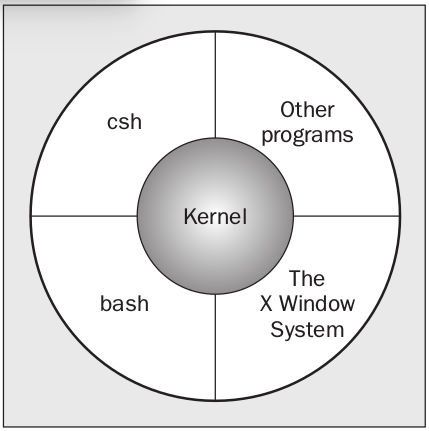
\includegraphics[width=.4\linewidth]{Figs/system.png}
  \end{center}
\end{frame}

\begin{frame}[fragile]{Programming in the Shell}
  \begin{itemize}
    \item The shell uses an interpreted language, parsing each
      statement as one or more programs with their arguments
    \item One of the main reasons to use the shell is you can do your
      job simply and quickly
    \item Batch processing, bulk conversion, etc. of files are just a
      short script away
    \item Shell scripts are used when efficiency may take a back hand
      whilst maintining a coherence work sequence comes to the fore
    \item They may be used to run commands in predetermined (even
      conditioned) sequences
  \end{itemize}
\end{frame}

\section{Syntaxes and Examples}
\begin{frame}[fragile]{Starting Off}
  \begin{columns}
    \begin{column}{0.3\textwidth}
      \textbf{A Sample Program}
\begin{verbatim}
#!/bin/sh

# A comment
for file in *
do
    echo $file
done

exit 0  
\end{verbatim}
    \end{column}
    \begin{column}{0.7\textwidth}
      \textbf{Notes}
      \begin{itemize}
        \item The first line of each script must contain the location
          to the shell program (\verb|sh| in this case) following
          \verb|#!|
        \item All statements following a \verb|#| are ignored as
          comments
        \item The \verb|exit| command produces a return value
        \item To make the script executable, run
\begin{verbatim}
sudo chmod +x script.sh
\end{verbatim}
        \item It is prudent to save shell scripts with a ``.sh''
          extension 
      \end{itemize}
    \end{column}    
  \end{columns}
\end{frame}

\subsection{Variables}
\subsection{An Example}
\begin{frame}[fragile]{Variables}
  \begin{itemize}
    \item By default variables are strings in Bash
    \item To assign a variable use the \verb|``=''| sign
\begin{verbatim}
$> var1=Hello
$> var2="Hello World"
\end{verbatim}
    \item Since by default space is the escape sequence, strings with
      space have to be enclosed in double quotes
    \item The value of a variable is accessed using the \verb+``$"+
      character. For example, to print the value of \verb+var2+ onto
      the screen we use,
\begin{verbatim}
$> echo "$var2"
\end{verbatim}
    \item To \textbf{read} from user input we use,
\begin{verbatim}
$> read var2
\end{verbatim}
    \item For outputting text as is use single quotes or precede the
      special characters by a backslash (\textbackslash{})
\end{itemize}
\end{frame}

\begin{frame}[fragile]{Environment Variables}
  \begin{itemize}
  \item Since the Linux system itself is presented through a Bash
    interface, there are several variables pre-defined in the
    ``environment''
  \item Most of them denote to particular file addresses to aid ease
    of access
  \item For example the variable \verb+HOME+ points to
    \verb+/home/nidish_ubuntu1604+ in my pc. It points to the home
    directory
  \item Another example would be the \verb|PATH| variable. It stores
    the locations the system searches in when programs are
    called. Programs stored in \verb|PATH| may be invoked with their
    names from anywhere in the system. \verb+$> echo $PATH$+ throws
    back in my system,
\begin{verbatim}
/home/nidish_ubuntu1604/bin:/usr/local/sbin:
/usr/local/bin:/usr/sbin:/usr/bin:/sbin:/bin:
/usr/games:/usr/local/games:/snap/bin:
/home/nidish_ubuntu1604/Tisean
\end{verbatim}
  \end{itemize}
\end{frame}

\begin{frame}[fragile]{Environment Variables}
  \begin{itemize}
  \item In some cases it may be necessary for us to \textbf{add} to
    existing variables without removing the current values
  \item For example, to add the path of a development folder to the
    \verb|PATH| we use,
\begin{verbatim}
$> export PATH="$PATH:$HOME/Development/bin"
\end{verbatim}
  \item This change will be valid only for the current terminal
    session. To make it global, you could type it into the file
    \verb|$HOME/.bashrc| (You need superuser privileges for this)
  \item Note that the \verb|.bashrc| file will not be visible in a
    graphical file explorer since the name starts with a "."
  \item To view all such configuration files, go to your terminal and
    use \verb|ls| with the \verb|-a| flag
\begin{verbatim}
$> cd $HOME
$> ls -a
\end{verbatim}
  \end{itemize}
\end{frame}

\begin{frame}[fragile]{Variables}{Operations on Variables}
  \begin{itemize}
  \item Almost all the scenarios where Bash scripting is necessary
    involve file conversions and other operations requiring the
    system to manipulate file names one by one
  \item We make a list of the most handy operations that may be
    performed on Variables. In all the below examples \verb+par+ is
    taken as a variable\\
    \begin{center}
      \begin{tabular}{|c|c|}
        \hline
        \verb|${par:-bar}|&Use value of \verb+par+ if it exists\\
                          &``bar'' if not\\\hline
        \verb|${par:=bar}|&Use value of \verb+par+ if it exists\\
                          &assign ``bar'' if not\\\hline
        \verb|${par:+bar}|&Return ``bar'' if par exists\\
                          &Not equalling to \verb+NULL+\\\hline
        \verb|${#par}|&Returns length of the variable\\\hline 
      \end{tabular}
    \end{center}
  \end{itemize}
\end{frame}

\begin{frame}[fragile]{Variables}{Formatting}
  \begin{itemize}
  \item We list some more operations
    \begin{center}
      \begin{tabular}{|c|c|}
        \hline
        \verb|${par%word}|&Returns \verb+$par+ with the\\
                    &smallest part from the end\\
                    &matching \verb|word| removed\\\hline
        \verb|${par%%word}|&Returns \verb+$par$+ with the\\
                    &longest part from the end\\
                    &matching \verb|word| removed\\\hline
        \verb|${par#word}|&Returns \verb+$par$+ with the\\
                      &smallest part from the beginning\\
                      &matching \verb|word| removed\\\hline
        \verb|${par##word}|&Returns \verb+$par$+ with the\\
                    &longest part from the beginning\\
                    &matching \verb|word| removed\\\hline
      \end{tabular}
    \end{center}
  \item These tend to come in very handy when we're dealing with
    converting a set of files and renaming them with appropriate
    extensions
  \end{itemize}
\end{frame}

\subsection{Parameters}
\begin{frame}[fragile]{Parameters}{Command-Line Arguments to Bash
    Scripts} 
  \begin{itemize}
  \item Command-line arguments may be passed to a Bash Script
  \item The following list the symbols that may be used to access
    information about the passed arguments 
    \begin{tabular}{|c|c|}
      \hline
      \verb|$#|&Number of Arguments passed\\
      \hline
      \verb|$0,$1,$2..|&zeroth argument(script name),\\
      &and other arguments\\
      \hline
      \verb|$*|&comma-separated list of all\\
      &the arguments(excluding script name)\\
      \hline
      \verb|$@|&space-separated list of all\\
      &the arguments(excluding script name)\\
      \hline
      \verb|IFS|&This stores the default field\\
      &separator used to parse the arguments\\
      \hline
    \end{tabular}
  \item There are ways to work with command line arguments more
    efficiently, for example by using the \verb|getopt| binary. We
    wiill not go into this presently
  \end{itemize}
\end{frame}

\subsection{Conditionals}
\begin{frame}[fragile]{Conditionals}
  \begin{itemize}
  \item In Bash all the variables are fundamentally strings denoting
    file/folder names. The conditionals are built around this.\\
    \textbf{The} \verb+test+ \textbf{Command}
  \item This command (refer the man page) returns $0$ if the condition
    is satisfied and $1$ if not. The \verb|if| command takes input in
    this format.
  \item Alternately, the \verb+test+ command may be called using the
    ``\verb|[|'' character. Closing the test statement using
    ``\verb|]|'' is a recommended practice.
  \item The options that may be passed to it are classified into,
    \begin{enumerate}
    \item File Conditionals
    \item String Conditionals
    \item Arithmetic Conditionals
    \end{enumerate}
  \end{itemize}
\end{frame}

\begin{frame}[fragile]{Conditionals}{The test Command}
  \begin{columns}
    \begin{column}{0.5\textwidth}
      \begin{center}
        \textbf{File Conditionals}\\
        \begin{tabular}{|c|c|}
          \hline \textbf{Call}&\textbf{True if}\\\hline
          [ -f file ]&regular file\\\hline
          [ -d file ]&directory\\\hline
          [ -x file ]&executable\\\hline
          [ -s file ]&size non-zero\\\hline
          [ -r file ]&readable\\\hline
          [ -w file ]&writable\\\hline
          [ -e file ]&exists\\\hline
        \end{tabular}
      \end{center}
    \end{column}
    \begin{column}{0.5\textwidth}
      \begin{center}
        \textbf{Arithmetic Conditionals}\\
        \begin{tabular}{|c|c|}
          \hline \textbf{Call}&\textbf{True if}\\\hline
          e1 -eq e2 & expressions equal\\\hline
          e1 -ne e2 & expressions inequal\\\hline
          e1 -lt e2 & lesser than\\\hline
          e1 -le e2 & lesser-equal\\\hline
          e1 -gt e2 & greater than\\\hline
          e1 -ge e2 & greater-equal\\\hline
          ! e1 & expression false\\\hline
        \end{tabular}
      \end{center}
    \end{column}
  \end{columns}
  \begin{center}
    \textbf{String Conditionals}\\
    \begin{tabular}{|c|c|}
      \hline \textbf{Call}&\textbf{True if}\\\hline
      s1 = s2 & strings equal\\\hline
      s1 != s2 & strings inequal\\\hline
      -n s1 & string not null\\\hline
      -z s1 & string null\\\hline
    \end{tabular}\\
  \end{center}
\end{frame}

\begin{frame}[fragile]{Conditionals}{An Example}
\begin{columns}
  \begin{column}{0.5\textwidth}
    \textbf{Example Program}\\
\begin{verbatim}
if test -f fred.c
then
    echo "FOUND!"
else
    echo "NOT FOUND!"
fi
# (equivalently)
if [ -f fred.c ]
then
    echo "FOUND!"
else
    echo "NOT FOUND!"
fi
\end{verbatim}
  \end{column}
  \begin{column}{0.5\textwidth}
    \textbf{Notes}
    \begin{itemize}
    \item The snippet shows two ways of conducting the same
      conditional using the \verb|if-then-else-fi| construct
    \item The statements check for the existence of the file
      ``fred.c'' and print ``FOUND!'' or ``NOT FOUND!'' onto the
      screen accordingly
    \item More examples are attached in an adjoining folder
    \end{itemize}
  \end{column}
\end{columns}
\end{frame}

\begin{frame}[fragile]{Conditionals}{The case-esac construct}
  \begin{itemize}
  \item \textbf{Syntax}\\
\begin{verbatim}
echo "Type yes :"
read var
case "$var" in
  [yY] | [yY][eE][sS] ) echo "Good Morning!";;
  [nN] | [nN][oO] ) echo "Bad Morning!";;
  * ) echo "Input not recognized";;
esac
\end{verbatim}
  \item The script checks if input is only "y" or "Y" or "yes" with
    whatever case in the first line
  \item In the second, it checks if the input is no or it's
    derivatives
  \item \verb|* )| denotes the default behavior
  \item Note the two semicolons ending each statement
  \end{itemize}
\end{frame}

\subsection{Loops}
\begin{frame}[fragile]{Loops}
  \begin{itemize}
  \item Loops are very useful in conducting repetitive processes over
    a similar set of files, strings or numbers
  \item A very useful command line utility is \verb|sed|, used to
    produce a set of equispaced numbers as one column
  \item For example, to produce numbers 1 through 10, the command is,
\begin{verbatim}
sed 1 1 10
\end{verbatim}
  \item The arguments are start number, spacing, and end number,
    respectively
  \item Bash has the \verb|for, while| and \verb|until| loop
    constructs
  \item In syntax, the \verb|while| and \verb|until| constructs are
    very similar
  \end{itemize}
\end{frame}

\begin{frame}[fragile]{Loops}{The for Loop Construct}
  \textbf{Syntax}\\
\begin{verbatim}
for <var_name> in <set_of_values>;
do
  <loop_body>
done
\end{verbatim}
  \begin{itemize}
  \item The for loop operates by assigning a variable by a fixed
    sequence of numbers
  \item For example, to list out a set of numbers, either of the
    following may be used
\begin{columns}
\begin{column}{0.3\textwidth}
\begin{verbatim}
for i in 1 2 3 4 5;
do
  echo $i;
done;
\end{verbatim}
\end{column}
\begin{column}{0.3\textwidth}
\begin{verbatim}
for i in `seq 1 1 5`;
do
  echo $i;
done;
\end{verbatim}
\end{column}
\end{columns}
  \end{itemize}
\end{frame}

\begin{frame}[fragile]{Loops}{The while Loop Construct}
  \textbf{Syntax}\\
\begin{verbatim}
while <test_statement>;
do
  <loop_body>
done
\end{verbatim}
  \begin{itemize}
  \item The \verb|while| construct works by evaluating the test
    statement and breaks the loop if it evaluates to false
  \item It is upto the user to ensure that the loop does not end up ad
    infinitum. An example,
\begin{verbatim}
read invar;
while [ "$invar" != "password" ]; do
  echo "Sorry, try again!"
  read invar
done
\end{verbatim}
  \end{itemize}
\end{frame}

\begin{frame}[fragile]{Loops}{The until Loop Construct}
  \textbf{Syntax}\\
\begin{verbatim}
until <test_statement>;
do
  <loop_body>
done
\end{verbatim}
  \begin{itemize}
  \item The \verb|until| construct works by evaluating the test
    statement and breaks the loop if it evaluates to true
  \item It is upto the user to ensure that the loop does not end up ad
    infinitum. An example,
\begin{verbatim}
read invar;
until [ "$invar" = "password" ]; do
  echo "Sorry, try again!"
  read invar
done
\end{verbatim}
  \end{itemize}
\end{frame}

\subsection{Lists}
\begin{frame}[fragile]{Lists}
  \begin{itemize}
  \item Often, we would like a set of statements to be evaluated in a
    particular secuence conditioned upon the behavior of the others
  \item In Bash, we have the \verb|AND| and the \verb|OR| lists whose
    functions are pretty obvious
  \item The \verb|AND| list is a set of statements separated by a
    \verb|&&| which will be executed from left to right upon
    successive return of true. If false is returned in any one
    statement, false is returned as the return value of the compound
    statement
  \item The \verb|OR| list is a set of statements separated by a
    \verb+||+ which will be executed from left to right until one
    succeeds
  \item Some striking examples may be found in the directory attached
    herewith 
  \end{itemize}
\end{frame}

\subsection{Functions}
\begin{frame}[fragile]{Functions}
    \textbf{Syntax}\\
\begin{verbatim}
<fn_name>() {
  local <local_var>=<val>;
  <fn_body>
  return <ret_val>;
}
\end{verbatim}
  \begin{itemize}
  \item A function is called by its name - arguments may be passed to
    it as command line arguments are passed while calling a regular
    program
  \item The \verb|echo| strings of a function may be captured into a
    separate variable during the call by \verb|res="$(func args)"|
  \item The return value of the last function called may be accessed
    through \verb|$?|
  \item The \verb|local| keyword may be used for local variables
  \item Check the adjoining folder for examples
  \end{itemize}
\end{frame}

\subsection{Commands}
\begin{frame}[fragile]{Commands}
  \begin{itemize}
  \item In \verb|bash|, in addition to normally encountered
    constructs, there are what are called, \verb|commands|
  \item These help in improving comfort in terms of short hands and
    other such constructs. We list some out here
  \item The \verb|eval| command may be used to evaluate the value of
    a variable who's name is stored in another variable,
  \item The \verb|:| command can replace \verb|true| for more
    efficient usage
    \begin{columns}
      \begin{column}{0.3\textwidth}
        {\centering \textbf{The eval command}}
\begin{verbatim}
foo=10
x=foo
eval y='$'$x
echo $y
\end{verbatim}
      \end{column}
      
      \begin{column}{0.4\textwidth}
        {\centering \textbf{The : command}}
\begin{verbatim}
if [ -f file ]; then
    :
else
    echo "Inexistant!"
fi
\end{verbatim}        
      \end{column}
    \end{columns}
  \end{itemize}
\end{frame}

\begin{frame}[fragile]{Commands}
  \begin{itemize}
  \item The \verb|exec <cmd_name> <args>| command may be used to
    replace the current shell with a different program
  \item The \verb|exit| command is used to return an exit value to the
    shell. Values -1 to 125 are blocked for programs and may be
    used. \emph{126 means teh file was not executable; 127 means a
      command was not found; 128 and above mean that a signal
      occurred}
  \item The \verb|export <var>| ensures that a variable defined in a
    shell script is available in any script called from the script
  \item The \verb|expr| command evaluates its arguments as an
    expression. In Bash, all arithmetic are done in integers. The
    following are equivalent
\begin{verbatim}
x=$(expr $x + 1)
x=`expr $x + 1`
x=&(($x+1))
\end{verbatim}
  \end{itemize}
\end{frame}

\begin{frame}[fragile]{Here Docs}{Write a script right here}
  \begin{itemize}
  \item In some situations, we might want to execute a script from
    another interpreter and we would like to have the script in the
    current one itself
  \item The \verb|here documents| come to our rescue. We set the
    program to be called, and an end string. All text written in
    between the first call and the end string are passed into the
    interpreter specified\\
    \begin{columns}
      \begin{column}{0.35\textwidth}
        \textbf{cat}\\
\begin{verbatim}
cat <<!FUNKY!
hello
this is a here
document
!FUNKY!
\end{verbatim}
      \end{column}
      \begin{column}{0.35\textwidth}
        \textbf{gnuplot}\\
\begin{verbatim}
gnuplot -p<<EOF
set grid
set zeroax lt -1
plot sin(x)
EOF
\end{verbatim}
      \end{column}
    \end{columns}
  \end{itemize}
\end{frame}

\begin{frame}{Thank You\footnote{Do check out the adjoining directory
      for a small introduction to GUI design with the dialog command}}
  \begin{itemize}
  \item The current tutorial was made in Ubuntu 16.04, Unity
  \item The presentation was typeset using Latex (Beamer)    
  \end{itemize}

  \textbf{Reference}
  \begin{thebibliography}{2}
    \bibitem{beg} Mathew, N. \& Stones, R. \emph{Beginning Linux
        Programming}, 3rd ed. Wiley Publishing, Inc., 2004 ISBN:
      0-7645-4497-7  
  \end{thebibliography}
\end{frame}

\end{document}
